\section{Technical Solution}
\label{sec:TechnicalSolution}
\subsection{Set-up}
\label{sub:Set-up}
The web-cam we have used to gather our data with is a Genius iSlim 321R that can take both regular and infra-red images.
Mounted to the web-cam is a plastic frame with 4 LED lights and 4 infra-red lights that are placed just besides the LED lights.
The LED and infra-red lights are controlled by a Phidget single board computer \cite{phidgets2012website}.
The LED lights have colours and are placed in the following pattern: Yellow-Red-Camera-Green-Yellow.
The web-cam set up can be seen on Figure~\ref{fig:webcamsetup}.

Our project is written in python 2.7 using the following libraries: 
\begin{itemize} %references?
\item{Scitkit-learn for machine learning algorithms \cite{scikitlearn2012website}.}
\item{OpenCV for image analysis and manipulation \cite{opencv2012website}.}
\item{Numpy for matrix manipulation, also required by some of the other libraries\cite{scipy2012website}.}
\item{Matplotlib for plotting results \cite{matplotlib2012website}.}
\item{Phidgets python API to control the LED- and infra-red lights.}
\end{itemize}

To control the mounted lights, we modified an example phidgets python-script by Adam Stelmack \cite{phidgetexample2012download}.

\subsection{Experiment}
\label{sub:Experiment}
To perform the actual experiment, first of all data must be gathered.
The initial scenarios we wanted to test were combinations of the head being fixated and looking at a point, the head moving while looking at a point, and the infra-red lights being turned on or off.
This leaves us with the 4 scenarios with-light-head-move (WLHM), no-lights-head-move (NLHM), with-lights-head-still (WLHS) and no-lights-head-still (NLHS).
Test-subjects were then asked to place their head at a set point and look at the different points. For images of our test-subjects, see figure \ref{fig:testsubjects}.%, \ref{fig:mikkertest2}, \ref{fig:spencertest}, \ref{fig:petertest} and \ref{fig:nielstest}.
We then recorded video sequences of about 5 seconds in length at 30 frames per second of the various scenarios and saved the videos with appropriate names according to the scenarios.

\begin{figure}[h!]
\centering
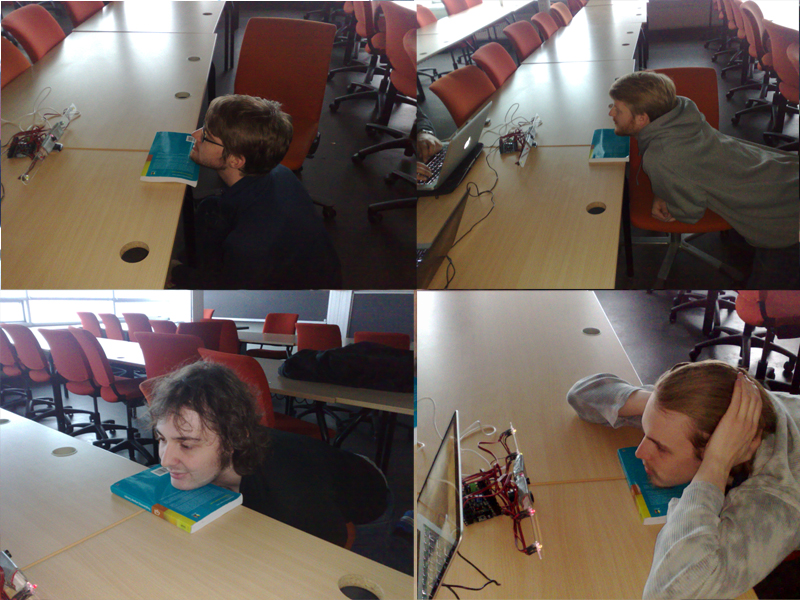
\includegraphics[width=0.8\textwidth]{testsubjects}
\caption{Data gathering on test-subjects.}
\label{fig:testsubjects}
\end{figure}

Images were then extracted from the videos every 10 frames using OpenCV and named in such a way it was easy to identify the scenario and the frame it was from.
Bad images, such as frames were the eyes were obscured or closed, were then manually filtered out and added to an ignore-file.
To see some of the images and the eyes that were extracted from them, see figure \ref{fig:experimentimage}.

\begin{figure}[h!]
\centering
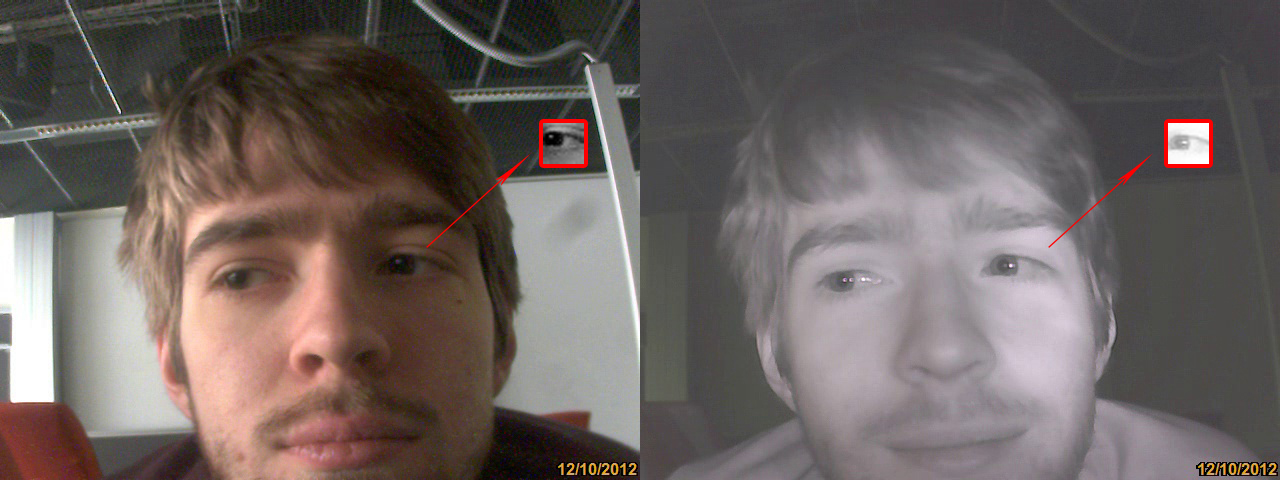
\includegraphics[width=0.8\textwidth]{ExperimentImages}
\caption{Images of a test subject with infra-red light being on and off and the grayscale eye-images extracted from them.}
\label{fig:experimentimage}
\end{figure}

The corners of the eye and the centre of the pupil were then marked manually using OpenCV and the three points were saved to meta-data files.
This data can be used for feature based learning, though more information such as glints may be desirable.

For high-dimensional learning, we also needed to separate the eye images.
To do this, eye images were extracted from the larger images using the previously marked points.
To extract the image, the images were loaded and converted to grayscale.
They were then histogram-equalized to broaden the contrast in the image. %skriv noget om effekt på læring?
The eye was then sliced out of the larger image and rescaled to a desired size, such as $20\times 20$, $40\times 40$ or $60\times 60$, and then saved.
This provided us a good starting point for analysing the eye images with PCA, and applying machine learning techniques on them.
